%%%%%%%%%%%%%%%%%%%%%%%%%%%%%%%%%%%%%%%%%%%%%%%%%%%%%%%%%%%%%%%%%%%%%%%%%%%%%%%
\section{Flux Separability Approximation}
\label{sec:flux-separability}
%%%%%%%%%%%%%%%%%%%%%%%%%%%%%%%%%%%%%%%%%%%%%%%%%%%%%%%%%%%%%%%%%%%%%%%%%%%%%%%

first paragraph: intro neutron transport eqn
-balance equation between streaming, collisions, scattering and fission production
-intro terms, $k$ for spatial zone and $g$ for energy group index, etc.

second paragraph: multi-group approx.
-apply multi-group approx.
-integrate across discrete energy groups
-introduce multi-group form of transport eqn

third paragraph: multi-group constants
-scattering: Moment expansion of the scattering kernel leads to 
-fission: angular distribution of outgoing neutrons is iso-in-lab
-total mgxs: to preserve the group-wise reaction rates, must collapse with angular flux
  -segue into flux separability approximation

fourth paragraph: flux separability approximation
-re-use section from thesis
-interchange scalar flux for angular flux in collapse of total multi-group cross section

fifth paragraph: introduce figures
-\autoref{fig:incoming-outgoing} 
-\autoref{fig:batman-plots-a}
-\autoref{fig:batman-plots-b}
-although the MGXS varies greatly depending on the angle incident on a fuel pin spatial zone, this variation is typically neglected altogether in MGXS
-this paper quantifies the impact of neglecting this angular variation by using scalar flux-weighted MGXS

\begin{dmath}
\label{eqn:transport-eqn-ce}
\mathbf{\Omega} \cdot \nabla \psi(\mathbf{r},\mathbf{\Omega},E) + \Sigma_{t}(\mathbf{r},E)\psi(\mathbf{r},\mathbf{\Omega},E) = \int\displaylimits_{0}^{\infty}\int\displaylimits_{4\pi} \Sigma_{s}(\mathbf{r},{\mathbf{\Omega'}\rightarrow\mathbf{\Omega}},{E'\rightarrow E}) \psi(\mathbf{r},\mathbf{\Omega'},E') \mathrm{d}\mathbf{\Omega'} \mathrm{d}E' + \frac{1}{4\pi k_{eff}}\int\displaylimits_{0}^{\infty}\int\displaylimits_{4\pi} \nu\Sigma_{f}(\mathbf{r},{E'\rightarrow E})\psi(\mathbf{r},\mathbf{\Omega'},E') \mathrm{d}\mathbf{\Omega'} \mathrm{d}E'
\end{dmath}

\begin{dmath}
\label{eqn:transport-eqn-mg}
\mathbf{\Omega} \cdot \nabla \psi_{g}(\mathbf{r},\mathbf{\Omega}) + \Sigma_{t,g}(\mathbf{r},\mathbf{\Omega})\psi_{g}(\mathbf{r},\mathbf{\Omega}) =
\frac{1}{4\pi}\sum_{g'=1}^{G} \Sigma_{s,g' \rightarrow g}(\mathbf{r}) \phi_{g'}(\mathbf{r}) + \frac{1}{4\pi k_{eff}}\sum_{g'=1}^{G} \nu\Sigma_{f,g' \rightarrow g}(\mathbf{r})\phi_{g'}(\mathbf{r})
\end{dmath}


The first term on the left hand side of the equation represents the streaming of neutrons within space and the second term is the total neutron collision rate determined by the total cross section $\Sigma_{t}$. On the right hand side, the first term models the scattering of neutrons at some energy $E'$ and direction $\mathbf{\Omega'}$ into energy $E$ and direction $\mathbf{\Omega}$. 

The multi-group approach used to solve the transport equation subdivides the neutron's energy into discrete bins known as energy groups. The energy groups are indexed starting at 1 for high energies and ending with $G$ for the lowest energies of interest. The MGXS are the averages of the corresponding continuous energy cross sections weighted by the angular neutron flux $\psi$ in each energy group:

\begin{dmath}
\label{eqn:sigt-mg}
\Sigma_{t,g}(\mathbf{r},\mathbf{\Omega}) \equiv \frac{\int\displaylimits_{E_{g}}^{E_{g-1}} \Sigma_{t}(\mathbf{r},E)\psi(\mathbf{r},\mathbf{\Omega},E)\mathrm{d}E}{\int\displaylimits_{E_{g}}^{E_{g-1}} \psi(\mathbf{r},\mathbf{\Omega},E)}
\end{dmath}

The angular dependence of the total cross section is often treated with the flux separability approximation. Flux separability makes the simplifying assumption that the energy and angular dependence of the flux varies independently such that the angular flux can be written as the product of the scalar neutron flux $\phi(\mathbf{r},E)$ and some function $W(\mathbf{r}, \mathbf{\Omega})$:

\begin{dmath}
\label{eqn:flux-separate}
\psi(\mathbf{r},\mathbf{\Omega},E) = \phi(\mathbf{r},E) W(\mathbf{r},\mathbf{\Omega})
\end{dmath}

\noindent The angular dependence of the $\Sigma_{t,g}$ may then be eliminated by inserting~\autoref{eqn:flux-separate} into~\autoref{eqn:sigt-mg}, factoring out $W(\mathbf{r},\mathbf{\Omega})$ and writing $\Sigma_{t}$ in terms of the scalar flux:

\begin{dmath}
\label{eqn:sigt-mg-scalar}
\Sigma_{t,g}(\mathbf{r}) \approx \frac{\int\displaylimits_{E_{g}}^{E_{g-1}} \Sigma_{t}(\mathbf{r},E)\phi(\mathbf{r},E)W(\mathbf{r},\mathbf{\Omega})\mathrm{d}E}{\int\displaylimits_{E_{g}}^{E_{g-1}} \phi(\mathbf{r},E)W(\mathbf{r},\mathbf{\Omega})} = \frac{\int\displaylimits_{E_{g}}^{E_{g-1}} \Sigma_{t}(\mathbf{r},E)\phi(\mathbf{r},E)\mathrm{d}E}{\int\displaylimits_{E_{g}}^{E_{g-1}} \phi(\mathbf{r},E)}
\end{dmath}

Although flux separability is a simple and commonly used approach to reduce the complexity of the ``true'' multi-group total cross section, it is not always valid and may not preserve neutron balance.

The flux separability approximation will necessarily hold in infinite homogeneous media since the flux does not vary in angle or space. However, the flux may vary greatly by angle in a heterogeneous geometry with significant spatial self-shielding. For example, consider the flux from two different directions impinged upon a discretized spatial zone for one radial ring and angular sector in a fuel pin in~\autoref{fig:incoming-outgoing}. The epithermal flux entering from the moderator will be unshielded and will likely be quite similar to the $\nicefrac{1}{E}$ asymptotic spectrum. In contrast, the flux which traverses the fuel pin will be significantly depressed in the resonant groups. As a result, the reaction rates for the incoming flux will be greater than those for the outgoing flux in resonant groups, which would be reflected in angular-dependent total MGXS.

Gibson further investigated this issue by using the reference ultra-fine angular flux to compute angular-dependent MGXS. Some examples of the angular-dependent capture MGXS generated for two different FSRs shaded in dark gray are shown in~\autoref{fig:batman-plots}. The MGXS in the FSR at the fuel/moderator interface in~\autoref{fig:batman-plots-a} ranges from less than 5 to more than 50 barns for angles entering and leaving the fuel pin. The peaks near 60$^{\circ}$ and 120$^{\circ}$ are due to extra moderation experienced by neutrons streaming through the infinite rectilinear fuel pin lattice at those angles. The MGXS in FSRs in the interior of the fuel pin, such as the one shown in~\autoref{fig:batman-plots-b}, exhibit similar but less prominent properties since the flux is shielded in all directions.

\begin{figure}[h!]
  \centering
  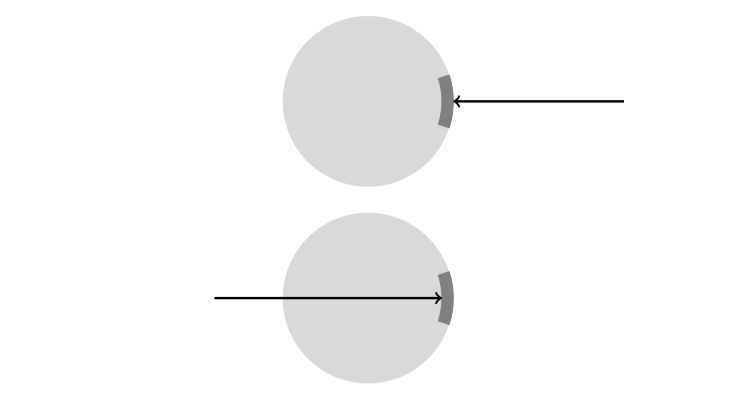
\includegraphics[width=\linewidth]{figures/incoming-outgoing}
  \caption{Angular flux impinged on an FSR from the moderator (top) and after traversing the fuel (bottom) \citep{gibson2016thesis}.}
\label{fig:incoming-outgoing}
\end{figure}

\begin{figure}[h!]
\begin{subfigure}{.45\textwidth}
  \centering
  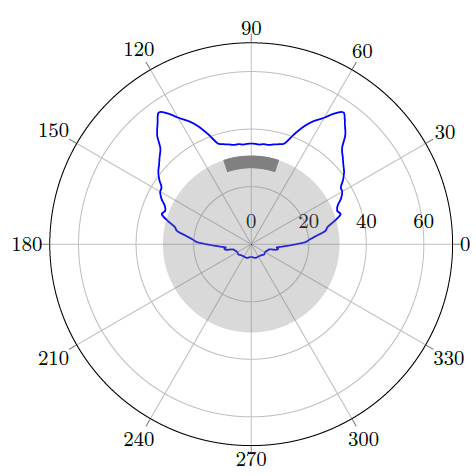
\includegraphics[width=0.9\linewidth]{figures/batman-1}
  \caption{}
  \label{fig:batman-plots-a}
\end{subfigure}
\begin{subfigure}{.45\textwidth}
  \centering
  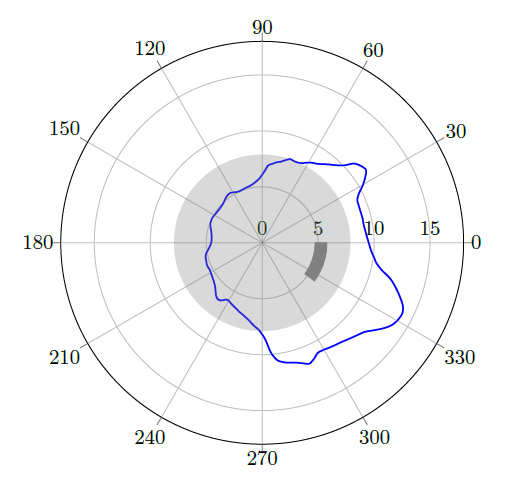
\includegraphics[width=0.9\linewidth]{figures/batman-2}
  \caption{}
  \label{fig:batman-plots-b}
\end{subfigure}
\caption{Angular-dependent capture MGXS for the 6.67 eV resonance group as a function of azimuthal angle for two different FSRs \citep{gibson2016thesis}. The radial axis is given in units of barns and the azimuthal axis in units of degrees.}
\label{fig:batman-plots}
\end{figure}
